\section{Implementation}
\indent Using the design structure above, our next aim was to create a code which had an independant and portable structure. This section describes how our design translated into code. This section is divided into two subsection; significant implementations and software testing.

\subsection{Significant Implementaion}

\subsubsection{Map and Cell class}
\indent Using the design structure discussed above we proceeded to the next phase - implementation. The implementation rests heavily on the idea of a matrix (used in the \texttt{Map} class) and the design of it's elements. The matrix can be thought of as holding an ordered pair of elements which are objects of the class \texttt{Cell}. A cell is defined by it's \texttt{row}, \texttt{col} and \texttt{isOccupied} boolean value. To read the paramaters to create the map, we used the following external lbraries, 

\begin{enumerate}[itemsep=1pt]
\item jackson-annotations
\item jackson-core
\item jackson-databind 
\end{enumerate}

The class \texttt{Map} holds the an object of class \texttt{MyMap} where the information of the json configuration file is mapped to. The following snippet represents the two lines which were used for the mapping, 

\begin{lstlisting}[language=java]
  ObjectMapper mapper = new ObjectMapper();
  testMap = mapper.readValue(new FileReader(this.file), MyMap.class);
\end{lstlisting}

The bounds of the matrix for $x$ and $y$ were between
\begin{equation*}
 0 \le x \le \texttt{WIDTH} \textnormal{  and  }  0 \le y \le \texttt{HEIGHT}
\end{equation*}
 respectively. The dimentions of the map initially were $0 \leq x \leq 1200$ and $0 \leq y \leq 800$. In order to reduce the amount of computation required by each agent when checking the availability of the next element of the matrix a modification was necessary. A map is created with a hegiht, width and a tilesize. On creation of the map, the tilesize was used to normalize the height and width used to construct the map of cells, 

\begin{equation*}
0 \le x \le \texttt{mapWidth} = \frac{\texttt{WIDTH}}{\texttt{tileSize}}  \textnormal{    and     }  0 \le y \le \texttt{mapHeight} = \frac{\texttt{HEIGHT}}{\texttt{tileSize}}
\end{equation*}

When displaying the grid, it was done with the original dimensions, but resized by the value of \texttt{tileSize}. 
%insert figure matrix here
\begin{figure}[H]
    \centering
    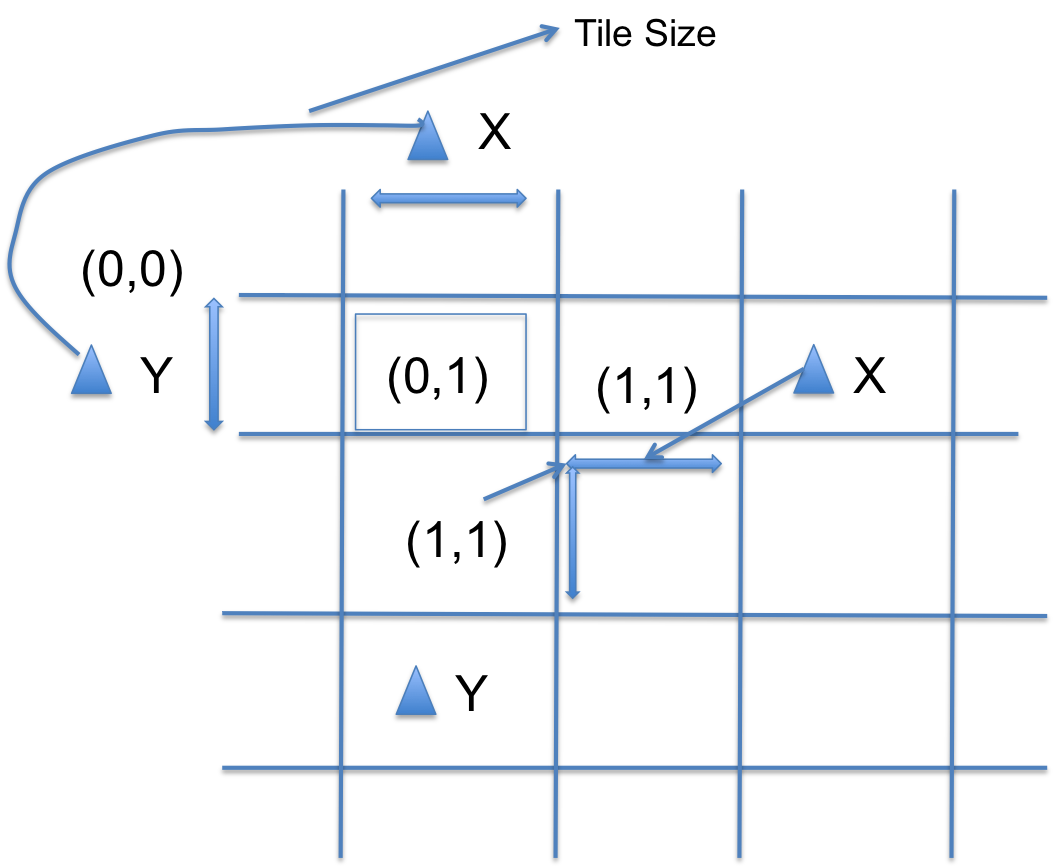
\includegraphics[width=0.8\textwidth]{pics/matrix.png}
    \caption{Expanding the GUI with tileSize}
    \label{fig:tileSize}
\end{figure}
In this way the creation of a map would hold $10^{2}$ less cells than the map which was displayed in the GUI. 

\subsubsection{JSON}
\indent  The json configuration file is used in the class \texttt{Map} the starting and ending positions of lanes, their id's and directions. It also holds the information of the lights and their default values. 

\begin{minipage}[b]{0.45\linewidth}
\centering
\begin{lstlisting}[language=json, firstnumber=1]
  ``lights'': [
    {
      ``state'': 1,
      ``position'': {
        ``row'': 42,
        ``col'': 64,
        ``occupied'': 0
      }
    }
    ...
  ]
\end{lstlisting}
%\caption{Lights in JSON file}
%\label{fig:jsonLights}
\end{minipage}
%%
\hspace{0.5cm}
\begin{minipage}[b]{0.45\linewidth}
\centering
\begin{lstlisting}[language=json, firstnumber=1]
  ``lanes'': [
  {
    ``id'': 3,
    ``direction'': 0,
    ``start'': {
      ``row'': 36,
      ``col'': 2
    },
    ``end'': {
      ``row'': 36,
      ``col'': 118
    }
  }
  ...
]
\end{lstlisting}
%\caption{Lanes in JSON file}
%\label{fig:jsonLanes}
\end{minipage}

\indent The above two code snippets describe the structure of the file. On startup the information in the configuration file would be read in class Map and mapped into the class \texttt{MyMap}. \texttt{MyMap} has methods which can then be accessed when needed by the other classes in the program. Using a json configuration file allowed for information to be easily parsed, and more importantly it allowed to keep all the map information in a single location. The latter point gave rise to a more dynamic code - if a new map was to be accessed a this could be done by using a seperate json file, leaving the rest of the code unmodified. 

\subsubsection{Car Class}


\indent In the method \texttt{move()}, it checks the direction of the car (all cases has the same functionality except how the car is checking if there is a car in front of it). It checks if there is a car in front of it by calling the \texttt{getCell()} of the class \texttt{Map}. If it not occupied it continue by checking if the getter \texttt{canMoveFromLights()} (main details will be found in a latter section). If it returns true it checks if it will turn (main details will be found in a latter section).Then it removes its previous position from the matrix, accelerate to its next position and then update the matrix. 

\indent The method accelerate checks the direction of the car and move it to its next position. It calculates its next position by this logic:

\[ \texttt{direction} = \left\{
  \begin{array}{l l}
    0 & \quad \text{then $x+=$ \texttt{tilesize}\*\texttt{speed} & and $y$ = $y$} \\
    1 & \quad \text{then $x-=$ \texttt{tilesize}\*\texttt{speed} & and $y$ = $y$} \\ 
    2 & \quad \text{then $y+=$ \texttt{tilesize}\*\texttt{speed} & and $x$ = $x$} \\ 
    3 & \quad \text{then $y-=$ \texttt{tilesize}\*\texttt{speed} & and $x$ = $x$} \\ 
    
  \end{array} \right.
\]

\indent Every time cars moves, its calling the boolean getter \texttt{canMoveFromLights()}, which returns if the car can move or not. When it returns that the car cannot move, this means that the car is in front of a light and the colour is red. First thing that this method does is to check the direction of the car. In all cases the method running a for loop of  the list of all the lights. If the positionof the light is the same of the cars (actually 1 point in front of the car) then it checks the colour of the light; if it is green it returns  true if it is red it returns false. The method \texttt{getCarImage()} checks the direction of the car and returns the current picture the car need to have.

\indent For a car to turn there is a condition, to be at a specific point $(x,y)$ in an intersection. This point exists after the every light. For the car to find this point it runs a for loop of all the lights of the map and searches for the current point. The calculation is done as follows, if


\[ \texttt{direction} = \left\{
  \begin{array}{l l}
    0 & \quad \text{and light's $x+1=$ car's $x$ \texttt{and light's $y=$ car's $y$}}\\
    1 & \quad \text{and light's $x-1=$ car's $x$ \texttt{and light's $y=$ car's $y$}}\\
    2 & \quad \text{and light's $y+1=$ car's $y$ \texttt{and light's $x=$ car's $x$}}\\
    3 & \quad \text{and light's $y-1=$ car's $y$ \texttt{and light's $x=$ car's $x$}}\\
    \end{array} \right.
\]


\indent When the car is at that point, then it makes a random decision to turn or go straight. If it makes the decision to turn then it changes its lane by calling the method setLane and passing as parameter a getter \texttt{getLane(laneID, laneDirection)} from the class \texttt{Map}. This getter has two parameters: the lane's id and direction that the car is moving now. This method passes this two variables to the \texttt{MyMap} class method \texttt{getCarNewLane()}. Finally this method calculates the new lane of the car by using this condition:


Let $L(i)$ be the current lane, $i-1$ the previous lane, $i+1$ the next line, $L(i)_{id}$ the id of the lane and $L(i)_{d}$ the direction:


\[ $L_{d}(i-1)$ = \left\{
  \begin{array}{l l}
    3 & \quad \text{and $L_{d}(i-1) = 2$ \texttt{then $L_{id}(i+1) = 3$  and $L_{d}(i+1) = 0$}}\\
    3 & \quad \text{and $L_{d}(i-1) = 0$ \texttt{then $L_{id}(i+1) = 4$  and $L_{d}(i+1) = 3$}}\\
    4 & \quad \text{and $L_{d}(i-1) = 3$ \texttt{then $L_{id}(i+1) = 4$  and $L_{d}(i+1) = 1$}}\\
    4 & \quad \text{and $L_{d}(i-1) = 1$ \texttt{then $L_{id}(i+1) = 3$  and $L_{d}(i+1) = 2$}}\\
    \end{array} \right.
\]


After that the car continues to move in its new direction




%----------------------------------------------------------------------------------------------------------------------------------------------------------------------------------
\subsection{Software Testing}

\indent This section will describe the software testing technique strategy in order to validate and verify the quality of the traffic simulation software; the testing techniques are classified into black-box and white box testing. The black-box and white-box testing will be in every part of the software implementation life cycle.

 \subsubsection{White box testing}
\indent White box testing also known as glass box testing and clear box testing is approach used for debugging of the software where the tester has excellent understanding of the design, structure and the  implementation of the software . In the white-box testing the tester selects random numbers for the input to examine various paths through the program in order determine the required output for the system. One of the advantages of white-box testing is that the tester does not require having a GUI in order to do this testing. There are various methods of white box testing such as unit testing, integration testing and system testing, however the main testing carried out in this project will be unit testing \cite{mauro}.

\subsubsection{Unit testing}
\indent The main testing technique used in the white-box testing in the traffic simulation is the unit testing, where the programmer?s carries out this testing. In the unit testing, component and unit of the code are tested. Where every component or unit of the code contains a small portion of the code, which is usually no longer than the class, a unit usually has few inputs and generates a single output \cite{mauro}.\newline

\textbf{Debugging 1}
\begin{enumerate}
\item {BUGS:} ArrayList bugs
\item Component tested: GamePanel
\item Unit tested: paint()
\item Test case1: for loop
\item Test case2: temporary Arrraylist
\end{enumerate} 

In white-box testing we found a lot of bugs and where they are originated. One of them was that when a car was leaving from the simulation?s map in the car component, it supposed to be removed from the ArrayList of cars. So in every move of the car, it checked if the location of the car was out of the map and, if true it was removed from the list; all that behaviour was placed inside of a loop in the list. But, when the program was running it crashed. However, after an exhaustive analysis of our code, we understood that the bug was created because the ArrayList was inside the loop. Eventually, we found a solution by making a method. This has a temporary empty arraylist that passes all elements of the main arrraylist to the temporary one, so the array does not go out of bound and the system does not crashed anymore. \newline

\textbf{Debugging 2}
\begin{enumerate}
\item {BUGS:} GamePanel
\item Component tested: GamePanel
\item Unit tested: paintMapOccupiedValues()
\item Test case1: If a cell RED $\implies$ cell is occupied %requires some special charaters
\item Test case2: If the cell GREEN $\implies$ the cell is unoccupied
\end{enumerate} 

Furthermore, other critical bug that we encountered was that when we created the matrix and the vision of the car, the agent car supposed stop when the car in front was also stopping. However this did not happened, and therefore caused an error. Consequently the bug there was that the car initialized one matrix for each and every one of the cars. The source of the problem was that each of the cars agents updated its own matrix, thus it was impossible to see if there was any other car in front of it. Nevertheless, we experimented with different solutions and found an effective one, which was to create a universal matrix and pass this matrix to each car.\newline

The paintGrid() method is used to paint the grid cells (which were made in the paint method). So If a cell is painted RED => the cell is occupied, and If the cell is printed GREEN => the cell is unoccupied. This helps us understand if the map is being updated properly. Moreover, it helps us understand if the agents, when moving, are setting their current grid occupied, when they are in it and when they leave - they are setting it as unoccupied. \newline

This method was very helpful to helps us see if the code is working properly and moreover, if the agents are working as they are they were programmed to. It basically, minimizes time spent on debugging - if we did not have it here, and in the event of a bug, we would have to sit through and debug the code for hours, but with this method, it saves a lot of time. \newline


\textbf{Debugging 3}
\begin{enumerate}
\item Component tested: Car
\item Unit tested: Accelerate()
\item Test case1: debug  =  true 
\item Test case2: debug   =  false
\end{enumerate} 

In order to make our white box testing more efficient we have used a preventing debugging approach. In the following case, the certain unit of code is being tested on the car component; car relies vastly on a Boolean value (debug) declared at the top, in order to function in an adequate way. For instance, when the system enters the accelerate method (), and if the value of variable debug is set to true, it will then follow the if (debug) statements, which give critical information, such as id of the lane to the map and hence allows the traffic to move in a respective way. However, if the value is set to false the program will continue without outputting the debugging information to the console.\newline

\textbf{Debugging 4}
\begin{enumerate}
\item Component tested: GamePanel
\item Unit tested: paintGrid(g2d)
\item Test case1: debug  =  true 
\item Test case2: debug   =  false
\end{enumerate} 

This method also helps us with the printing of the grid. A grid indicated the size an agent occupies in the game frame. The grid tells us if the agent moves properly/improperly/ as expected or in some unanticipated way.

 
%--------------------------------------------------
\subsection{Further Software Testing}
\indent This sub section discusses the bugs which where encountred and measures taken to minimize time spent finding them and the aids we used. 
\subsubsection{Debugging tools}
\indent The two debugging methods used were,  

\begin{enumerate}[itemsep=1pt]
\item \texttt{paintGrid()}
\item \texttt{paintMapOccupiedValues}
\end{enumerate}

Both tools were used as debbugging aids. The first method divided the grid into squares with the specified \texttt{WITDH} and \texttt{HEIGHT} of the map. This allowed to see if the proper cell was being occupied as an agent moved through the map. The second method would paint a cell red, if occupied and green if unnocupied giving a visual representation of the location of the agent on the board whether they were moving through the cells and if the correct cells were being occupied. These visual aids helped us significantly in identifying bugs which we were aware of and bugs which were lerking in the shadows and identified with this visual aid. 

%\subsection{Performcance Issues and Solutions}

\subsubsection{Block box testing}
 The black-box testing is one major part of the software implantation testing, it result in reliable functional validity of the system. In this project black-box testing has been done based on the requirement set at the beginning of the project, where any incomplete or any inconsistence behaviour can be simply detected .The black-box testing comes from the perspective of the users and it can take inputs that are either valid or invalid from the user perspective \cite{boris}. \newline
 
The black-box testing is carried out in every phase of project implementation and validation life cycle. In this project all testers were taking part of the black-box testing process, the tester where required to take part in the requirement and analysis phase and produce a plane in the design phase of the project  to meet the requirement throughout the black-box testing \cite{boris}. \newline
 
One of the advantages of the black-box testing is that the tester does not require have any knowledge of the software implementation within the software. In the black-box testing the programmers and the tester work independently. Another advantage of black-box testing is that it exposes any inconsistencies or any ambiguities in the specification requirement \cite{boris}. \newline
 
 \subsubsection{Functional testing }

One of the approaches used in the black-testing is known as the functional testing, where the testing is carried out based on the requirements of the project .In this testing the tester does not require to have a knowledge of the software implantation and the main purpose of functional testing is to acknowledge the user point of view on the finished traffic simulation product \cite{mauro}.


\subsubsection{Trafic simulation blackbox testing}

Due to the fact that this program has few controllers, a bug was found during the phase of the black box testing. The start button was pressed and the simulation was running after a different map is selected and the start button is pressed again both of them are running. The solution to this bug was to check if the GamePanel object is null before start running the simulation. If it was not null it removed the previous one from the Frame.









